% ---------------------------------------------------------------------
% -------------- PREAMBLE ---------------------------------------------
% ---------------------------------------------------------------------
\documentclass[12pt,a4paper,finnish,oneside]{article}
%\documentclass[12pt,a4paper,finnish,twoside]{article}
%\documentclass[12pt,a4paper,finnish,oneside,draft]{article} % luonnos, nopeampi

% Valitse 'input encoding':
%\usepackage[latin1]{inputenc} % merkistökoodaus, jos ISO-LATIN-1:tä.
\usepackage[utf8]{inputenc}   % merkistökoodaus, jos käytetään UTF8:a
% Valitse 'output/font encoding':
%\usepackage[T1]{fontenc}      % korjaa ääkkösten tavutusta, bittikarttana
\usepackage{ae,aecompl}       % ed. lis. vektorigrafiikkana bittikartan sijasta
% Kieli- ja tavutuspaketit:
\usepackage[english,swedish,finnish]{babel}
% Kurssin omat asetukset aaltosci_t.sty:
\usepackage{aaltosci_t}
% Jos kirjoitat muulla kuin suomen kielellä valitse:
%\usepackage[finnish]{aaltosci_t}           
%\usepackage[swedish]{aaltosci_t}           
%\usepackage[english]{aaltosci_t}           
% Muita paketteja:
\usepackage{alltt}
\usepackage{amsmath}   % matematiikkaa
\usepackage{calc}      % käytetään laskurien (counter) yhteydessä (tiedot.tex)
\usepackage{eurosym}   % eurosymboli: \euro{}
\usepackage{url}       % \url{...}
\usepackage{hyphenat}  % tavutuksen viilaamiseen liittyvä (hyphenpenalty,...)
\usepackage{supertabular,array}  % useampisivuinen taulukko

\newcommand{\scmrobo}{\textsc{Scheme-robo}}

% Koko dokumentin kattavia asetuksia:
%\hyphenation{vää-rin me-ne-vi-en eri-kois-ten sa-no-jen tavu-raja-ehdo-tuk-set}
% paikallisesti voi myös ta\-vut\-taa 

% Rangaistaan tavutusta (ei toimi?! Onko hyphenat-paketti asennettu?)
\hyphenpenalty=10000   % rangaistaan tavutuksesta, 10000=ääretön
\tolerance=1000        % siedetään välejä riveillä
% titlesec-paketti auttaa, jos tämän mukana menee sekaisin

% Rivivälin muuttaminen:
\linespread{1.24}\selectfont               % riviväli 1.5
%\linespread{1.24}\selectfont               % riviväli 1, kun kommentoit pois

% ---------------------------------------------------------------------
% -------------- DOCUMENT ---------------------------------------------
% ---------------------------------------------------------------------

\begin{document}

% -------------- Tähän dokumenttiin liittyviä valintoja  --------------

%\raggedright         % Tasattu vain vasemmalta, ei tavutusta
% ----------------- joitakin makroja ----------------------------------
%
% \newcommand{\sinunKomentosi}[argumenttienMäärä]{komennot%
% voiJakaaRiveille%
% jaArgumenttienViittaus#1,#2,#argumenttienMäärä}

% Joskus voi olla tarpeen kommentoida jotakin. Ei suositella. 
% Äläkä unohda lopulliseen! 
\newcommand{\Kommentti}[1]{\fbox{\textbf{OMA KOMMENTTI:} #1}}
% Käyttö: Kilometri on 1024 metriä. \Kommentti{varmista tämä vielä}.
% Eli newcommand:n komentosanan jälkeen hakasaluissa argumenttien lkm,
%  ja argumentteihin viitataa #1, #2, ...

%  Comment out this \DRAFT macro if this version no longer is one!  XXX
%\newcommand{\DRAFT}{\begin{center} {\it DRAFT! \hfill --- \hfill DRAFT!
%\hfill --- \hfill DRAFT! \hfill --- \hfill DRAFT!}\end{center}}

%  Use this \DRAFT macro in the final version - or comment out the 
%  draft-command
% \newcommand{\DRAFT}{~}

% %%%%%%%% MATEMATIIKKA %%%%%%%%%%%%%%%%%

% Määrätty integraali
\newcommand{\myInt}[4]{%
\int_{#1}^{#2} #3 \, \textrm{d}{#4}}

% http://kapsi.fi/jks/satfaq/
%\newcommand{\vii}{\mathop{\Big/}}
%\newcommand{\viiva}[2]{\vii\limits_{\!\!\!\!{#1}}^{\>\,{#2}}}
%%\[ \intop_0^{10} \frac{x}{x^2+1} \,\mathrm{d}x
%%= \viiva{0}{10} \frac{1}{2}\ln(x^2+1) \]

% matht.sty, Simo K. Kivelä, 01.01.2002, 07.04.2004, 19.11.2004, 21.02.2005
% Kokoelma matemaattisten lausekkeiden kirjoittamista helpottavia
% määrittelyjä.

% 07.04.2004 Muutama lisäys ja muutos tehty: \ii, \ee, \dd, \der,
% \norm, \abs, \tr.
%
% 19.11.2004 Korjattu määrittelyjä: \re, \im, \norm;
% lisätty \trp (transponointi), \hrm (hermitointi), \itgr (rakenteellinen
% integraali), ympäristö Cmatrix (hakasulkumatriisi);
% vanha transponointi \tr on mukana edelleen, mutta ei suositella.

% Pakotettu rivinvaihto, joka voidaan tarvittaessa määritellä
% uudelleen: 

%\newcommand{\nl}{\newline}

% Logiikan symboleja (<=> ja =>) hieman muunnettuina:

%\newcommand{\ifftmp}{\;\Leftrightarrow\;}
%\newcommand{\impltmp}{\DOTSB\;\Rightarrow\;}

% 'siten, että' -lyhenne ja hattupääyhtäläisyysmerkki vastaavuuden
% osoittamiseen: 

%\newcommand{\se}{\quad \text{siten, että} \quad}
%\newcommand{\vs}{\ {\widehat =}\ }

% Lukujoukkosymbolit:

%\newcommand{\N}{\ensuremath{\mathbb N}}
%\newcommand{\Z}{\ensuremath{\mathbb Z}}
%\newcommand{\Q}{\ensuremath{\mathbb Q}}
%\newcommand{\R}{\ensuremath{\mathbb R}}
%\newcommand{\C}{\ensuremath{\mathbb C}}

% Reaali- ja imaginaariosa, imaginaariyksikkö:

%\newcommand{\re}{\operatorname{Re}}
%\newcommand{\im}{\operatorname{Im}}
%\newcommand{\ii}{\mathrm{i}}

% Differentiaalin d, Neperin luku:

%\newcommand{\dd}{\mathrm{d}}
%\newcommand{\ee}{\mathrm{e}}

% Vektorimerkintä, joka voidaan tarvittaessa määritellä uudelleen
% (tämä tekee vektorit lihavoituina):

%\newcommand{\V}[1]{{\mathbf #1}}

% Kulmasymboli:

%\renewcommand{\angle}{\sphericalangle}

% Vektorimerkintä, jossa päälle pannaan iso nuoli;
% esimerkiksi \overrightarrow{AB} (tämmöisiä olemassaolevien
% symbolien uudelleenmäärittelyjä ei kyllä pitäisi tehdä):

%\renewcommand{\vec}[1]{\overrightarrow{#1}}

% Vektoreiden vastakkaissuuntaisuus:

%\newcommand{\updownarrows}{\uparrow\negthinspace\downarrow}

% Itseisarvot ja normi:

%\newcommand{\abs}[1]{{\left\vert#1\right\vert}}
%\newcommand{\norm}[1]{{\left\Vert #1 \right\Vert}}

% Transponointi ja hermitointi:

%\newcommand{\trp}[1]{{#1}\sp{\operatorname{T}}}
%\newcommand{\hrm}[1]{{#1}\sp{\operatorname{H}}}

% Vanha transponointi; jäljellä yhteensopivuussyistä, ei syytä käyttää.
%\newcommand{\tr}{{}^{\text T}}

% Arcus- ja area-funktiot, jossa päähaara osoitetaan nimen päälle
% vedetyllä vaakasuoralla viivalla (alkaa olla vanhentunutta,
% voitaisiin luopua):

%\newcommand{\arccot}{\operatorname{arccot}}
%\newcommand{\asin}{\operatorname{\overline{arc}sin}}
%\newcommand{\acos}{\operatorname{\overline{arc}cos}}
%\newcommand{\atan}{\operatorname{\overline{arc}tan}}
%\newcommand{\acot}{\operatorname{\overline{arc}cot}}

%\newcommand{\arsinh}{\operatorname{arsinh}}
%\newcommand{\arcosh}{\operatorname{arcosh}}
%\newcommand{\artanh}{\operatorname{artanh}}
%\newcommand{\arcoth}{\operatorname{arcoth}}
%\newcommand{\acosh}{\operatorname{\overline{ar}cosh}}

% Signum, syt, pyj:

%\newcommand{\sg}{\operatorname{sgn}}
%\renewcommand{\gcd}{\operatorname{syt}}
%\newcommand{\lcm}{\operatorname{pyj}}

% Lyhennemerkintöjä: derivaatta, osittaisderivaatta, gradientti,
% derivaattaoperaattori, vektorin komponentti, integraalin ylä- ja
% alasumma, Suomessa (ja Saksassa?) käytetty integraalin sijoitus-
% merkintä, integraali (rakenteellinen määrittely):

%\newcommand{\der}[2]{\frac{\dd #1}{\dd #2}}
%\newcommand{\osder}[2]{\frac{\partial #1}{\partial #2}}
%\newcommand{\grad}{\operatorname{grad}}
%\newcommand{\Df}{\operatorname{D}} 
%\newcommand{\comp}{\operatorname{comp}}
%\newcommand{\ys}[1]{\overline S_{#1}}
%\newcommand{\as}[1]{\underline S_{#1}}
%\newcommand{\sijoitus}[2]{\biggl/_{\null\hskip-6pt #1}^{\null\hskip2pt #2}} 
%\newcommand{\itgr}[4]{\int_{#1}^{#2}#3\,\dd #4}

% Matriiseja, joille voidaan antaa alkioiden sijoittamista sarakkeen
% vasempaan tai oikeaan reunaan tai keskelle osoittava lisäparametri
% (l, r tai c); ympärillä kaarisulut, hakasulut, pystyviivat (determinantti)
% tai ei mitään;
% esimerkiksi \begin{cmatrix}{ll}1 & -1 \\ -1 & 1 \end{cmatrix}:

%\newenvironment{cmatrix}[1]{\left(\begin{array}{#1}}{\end{array}\right)}
%\newenvironment{Cmatrix}[1]{\left[\begin{array}{#1}}{\end{array}\right]}
%\newenvironment{dmatrix}[1]{\left|\begin{array}{#1}}{\end{array}\right|}
%\newenvironment{ematrix}[1]{\begin{array}{#1}}{\end{array}}

% Kaunokirjoitussymboli:

%\newcommand{\Cal}{\mathcal}

% Isokokoinen summa:

%\newcommand{\dsum}[2]{{\displaystyle \sum_{#1}^{#2}}}

% Tuplaintegraali umpinaisen pinnan yli; korvataan jos parempi löytyy:
%\newcommand\oiint{\begingroup
% \displaystyle \unitlength 1pt
% \int\mkern-7.2mu
% \begin{picture}(0,3)
%   \put(0,3){\oval(10,8)}
% \end{picture}
% \mkern-7mu\int\endgroup}
       % Haetaan joitakin makroja

\selectlanguage{finnish}
\pagestyle{plain}
\pagenumbering{arabic}

% ---------------------------------------------------------------------
% -------------- Luettelosivut alkavat --------------------------------
% ---------------------------------------------------------------------

% -------------- Nimiölehti ja sen tiedot -----------------------------
%
% Nimiölehti ja tiivistelmä kirjoitetaan seminaarin mukaan joko
% suomeksi tai ruotsiksi (ellei erityisesti kielenä ole englanti). 
% Tiivistelmän voi suomen/ruotsin lisäksi kirjoittaa halutessaan
% myös englanniksi. Eli tiivistelmiä tulee yksi tai kaksi kpl.
%
% "\MUUTTUJA"-kohdat luetaan aaltosci_t.sty:ä varten.

\author{Ferrix Hovi}

\title{Ohjelmointiharjoitusten turvallisuuden automaattinen arviointi} % 2-osainen otsikko:
%\title{\LaTeX{}-pohja kandidaatintyölle \\[5mm] Pitkiä rivejä kokeilun vuoksi.}

% Otsikko tiivistelmään. Jos lisäksi engl. tiivistelmä, niin viimeisin:
\TITLE{Ohjelmointiharjoitusten turvallisuuden automaattinen arviointi}
\ENTITLE{Automatic Security Assessment of Programming Assignments}
% 2-osainen otsikko korvataan täällä esim. pisteellä:
%\TITLE{\LaTeX{}-pohja kandidaatintyölle. Pitkiä rivejä kokeilun vuoksi.}

\DEPT{Tietotekniikan laitos}               % T
\ENDEPT{Department of Computer Science Engineering}     % T

% Vuosi ja päivämäärä, jolloin työ on jätetty tarkistettavaksi.
\YEAR{2011}
\DATE{5. toukokuuta 2011}
\ENDATE{May 5, 2011}

% Kurssin vastuuopettaja ja työsi ohjaaja(t)
\SUPERVISOR{Ma professori Tomi Janhunen}
\INSTRUCTOR{Dosentti Ari Korhonen}

\ENSUPERVISOR{Professor (tem) Tomi Janhunen}
\ENINSTRUCTOR{Docent Ari Korhonen}

\PAAAINE{Ohjelmistotuotanto ja -liiketoiminta}
\CODE{T3003}

\KEYWORDS{avain, sanoja, niitäkin, tähän, vielä, useampi, vaikkei, %
niitä, niin, montaa, oikeasti, tarvitse}
\ENKEYWORDS{key, words, the same as in FIN/SWE}

% Tiivistelmään tulevat sivumäärät. 
% Kirjoita lopulliset sivumäärät käsin tai kokeile koodia. 
%
% Ohje 14.11.2006, luku 4.2.5:
% - sivumäärä = tekstiosan (alkaen johdantoluvusta) ja 
%   lähdeluettelon sivumäärä, esim. "20"
% - jos liitteet, niin edellisen lisäksi liitteiden sivumäärä,
%   tyyli "20 + 5", jossa 5 sivua liitteitä 
% - HUOM! Tässä oletuksena sivunumerointi alkaa nimiölehdestä 
%   sivunumerolla 1. %   Toisin sanoen, viimeisen lähdeluettelosivun 
%   sivunumero EI ole sivujen määrä vaan se pitää laskea tähän käsin

\PAGES{20}          % 999 tekstisivua
%\PAGES{999 $+$ 123}  % 999 tekstisivua + 123 liitesivua

%\thispagestyle{empty}  % nimiölehdellä ei sivunumerointia; tyylin mukaan ei tehdäkään?!

\maketitle             % tehdään nimiölehti

% -------------- Tiivistelmä / abstract -------------------------------
% Lisää abstrakti kandikielellä (ja halutessasi lisäksi englanniksi).

% Edelleen sivunumerointiin. Eräs ohje käskee aloittaa sivunumeroiden
% laskemisen nimiösivulta kuitenkin niin, että sille ei numeroa merkitä
% (Kauranen, luku 5.2.2). Näin ollen ensimmäisen tiivistelmän sivunumero
% on 2. \maketitle komento jotenkin kadottaa sivunumeronsa.
\setcounter{page}{2}    % sivunumeroksi tulee 2

% Tiivistelmät tehdään viimeiseksi. 
%
% Tiivistelmä kirjoitetaan käytetyllä kielellä (JOKO suomi TAI ruotsi)
% ja HALUTESSASI myös samansisältöisenä englanniksi.
%
% Avainsanojen lista pitää merkitä main.tex-tiedoston kohtaan \KEYWORDS.

\begin{fiabstract}
Käytännön harjoittelulla on merkittävä rooli ohjelmoinnin opetuksessa ja
kurssit ovat usein suuria. Automaattisella arvostelulla on tässä suuri
oppimista tehostava vaikutus. Toisaalta tuntemattoman ohjelmakoodin
suorittaminen on aina riski. Tämä työ tutkii kahta TKK:lla kehitettyä
kotitehtävätarkistinta turvallisuusnäkökulmasta ja selvittää, voiko staattista
analyysiä lisäämällä parantaa näiden turvallisuutta. Lisäksi tutkitaan
opetettavan ohjelmointikielen vaikutusta tarkistimeen liittyviin riskeihin.

TKK:lla kehitetyt tarkistimet EXPACA ja {\scmrobo} ovat lähestymistavoiltaan
hyvin erilaisia. Edellinen suorittaa käännettyä ohjelmaa virtuaalikonsolissa
ja jälkimmäinen suorittaa Scheme-proseduuria metasirkulaarisessa tulkissa.
{\scmrobo} on onnistuneesti rajannut kielen riskialttiit ominaisuudet pois
eikä siinä siksi ole ilmeisiä turvallisuusriskejä. EXPACA suorittaa
täysimittaisia ohjelmia, jotka on toteutettu virhealttiilla kielillä. Tämän
takia staattisen analyysin lisäämisestä tarkistusprosessiin voisi olla hyötyä.

Staattiset analysaattorit antavat yleisesti ottaen niin paljon vääriä
hälytyksiä, ettei niiden käyttö automaattisessa arvostelussa ole mielekästä.
Pscan ja UNO ovat analysaattoreita, jotka havaitsevat yhteensä neljän tyyppisiä
ongelmia. Ne tuottavat keskimääräistä vähemmän vääriä hälytyksiä ja soveltuvat
mahdollisesti EXPACAn laajentamiseen.

Työssä havaitaan myös, että opetettavalla ohjelmointikielellä ja staattisen
analyysin opetuksella voi olla suuri merkitys opiskelijoiden tietämykselle
turvallisesta ohjelmointitavasta.
\end{fiabstract}

%\begin{svabstract}
%  Ett abstrakt hit 
%%(\languagename)
%\end{svabstract}

%\begin{enabstract}
%  Here goes the abstract. FIXME
%(\languagename)
%\end{enabstract}


% -------------- Alkusanat --------------------------------------------
% Suositus: ÄLÄ käytä kandidaatintyössä.
%
%\newpage
%\input{luku_alkusanat}
%\clearpage                     % luku loppuu, loput kelluvat tänne
%\newpage

% -------------- Symbolit ja lyhenteet --------------------------------
% Suositus: Käytä vasta kun paljon symboleja tai lyhenteitä.
%
%% -------------- Symbolit ja lyhenteet --------------
%
% Suomen kielen lehtorin suositus: vasta kun noin 10-20 symbolia
% tai lyhennettä, niin käytä vasta sitten.
%
% Tämä voi puuttuakin. Toisaalta jos käytät paljon akronyymejä,
% niin ne kannattaa esitellä ensimmäisen kerran niitä käytettäessä.
% Muissa tapauksissa lukija voi helposti tarkistaa sen tästä
% luettelosta. Esim. "Automaattinen tietojenkäsittely (ATK) mahdollistaa..."
% "... ATK on ..."
%
\section*{Käytetyt lyhenteet}
%\section{Abbreviations and Acronyms}

\begin{tabular}{p{0.2\textwidth}p{0.6\textwidth}}
2k/4k/8k mode & COFDM operation modes \\
3GPP  & 3rd Generation Partnership Project; Kolmannen sukupolven 
matkapuhelupalvelu \\ 
ESP & Encapsulating Security Payload; Yksi IPsec-tietoturvaprotokolla \\ 
\end{tabular}

Jos tarvitset useampisivuista taulukkoa, kannattanee käyttää 
esim. \verb!supertabular*!-ympäristöä, josta on kommentoitu esimerkki.


 
%\clearpage                     % luku loppuu, loput kelluvat tänne

% -------------- Kuvat ja taulukot ------------------------------------
% Kirjoissa (väitöskirja) on usein tässä kuvien ja taulukoiden listaus.
% Suositus: Ei kandityöhön.

% -------------- Sisällysluettelo / TOC -------------------------------

\tableofcontents

\label{pages:prelude}
\clearpage                     % kappale loppuu, loput kelluvat tänne, sivunv.
%\newpage

% ---------------------------------------------------------------------
% -------------- Tekstiosa alkaa --------------------------------------
% ---------------------------------------------------------------------

% Muutetaan tarvittaessa ala- ja ylätunnisteet
%\pagestyle{headings}          % headeriin lisätietoja
%\pagestyle{fancyheadings}     % headeriin lisätietoja
%\pagestyle{plain}             % ei header, footer: sivunumero

% Sivunumerointi, jos käytetty 'roman' aiemmin
% \pagenumbering{arabic}        % 1,2,3, samalla alustaa laskurin ykköseksi
% \thispagestyle{empty}         % pyydetty ensimmäinen tekstisivu tyhjäksi

% input-komento upottaa tiedoston 

% --------------------------------------------------------------------

\section{TIK.kand -- kirjoittaminen \LaTeX{}:lla}
\label{sec:esimluku}

Tämä teksti on peräisin TIK.kand-kurssin historiallisesta \LaTeX{}-pohjasta,
jota kurssin koordinaattori Jukka Parviainen päivitti tammikuussa 2011.
Lisäksi suomen kielen lehtori Sanni Heintzmann kirjoitti rakenteellisia
vinkkejä lukuun~\ref{sec:tekstin_osat}. 

Pura zip-paketti ja katso ja muokkaa tex- ja bib-tiedostoja vapaasti.
Yritä olla koskematta sty- ja bst-tiedostoihin.

\subsection{Rakenne- ja muotoseikat}

Yleiset kandidaatintyön muotovaatimukset on annettu 
TKK:n kandidaattityöryhmän päätöksellä 14.11.2006%
\footnote{\url{http://www.tkk.fi/fi/opinnot/opintohallinto/paatokset/kandi20061114.pdf}}.

\textbf{TIK.kand suositus:} Lue nämä ohjeet erityisesti silloin, jos
et kirjoita työtä annettua \LaTeX{}-pohjaa käyttäen.

Näissä annetaan ohjeet työn rakenteelle (luku 3) ja muotoseikoille (luku 4):
%
\begin{quotation}
\noindent \it
Kandidaatintyö voi perustua teoreettisen taustan tarkasteluun 
ja sen analysointiin sekä johtopäätösten tekoon tai kokeelliseen osioon ja 
tulosten analysointiin sekä johtopäätösten tekoon
tai edellisten yhdistelmään.
Kandidaatintyön rakenteen tulee olla hyvän tieteellisen kirjoittamisen 
käytännön mukainen
ja sisältävän vähintään seuraavat osat: [$\ldots$] (Luku 3)
\end{quotation}

Rakenteen osia ovat: nimiölehti, tiivistelmä, sisällysluettelo,
symboli- ja lyhenneluettelo (työn luonteen vaatiessa voi puuttua),
johdanto, aikaisempi tutkimus (työn luonteen vaatiessa teoreettinen
tausta), tutkimusongelma ja -menetelmät, tulokset, tarkastelu (työn
luonteen vaatiessa johtopäätökset tai näiden yhdistelmä), lähteet,
liitteet (jos tarpeen). Osat johdannosta tarkasteluun muodostavan työn
tekstiosan. (Luku 3) Tekstiosan sopiva pituus on 15--20 sivua eikä
työtä ole syytä tarpeettomasti pidentää (luku 4.2.1).

Muotoseikoissa otetaan esille, että työn tulee olla jäsennelty
ja tyylillisesti sekä kielellisesti viimeistelty ja moitteeton.
Tarpeettomia tyylillisiä erikoisuuksia tulee välttää.
Tekstiosassa tulee olla vain työn kannalta oleelliset kuvat
tai taulukot. (Luku 4.1)
%
Kirjasinlaji tulee olla roomalaistyyppinen (Times New Roman
tai Computer Modern\footnote{\LaTeX{}}) ja kooltaan 12 pistettä
(luku 4.2.2). 
%
Työn nimessä ei saa esiintyä lyhenteitä, kaavoja tai lainauksia
(luku 4.2.3).

Nimiölehdellä tulee olla tiedot yliopistosta, tutkinto-ohjelmasta,
työn nimestä, luonteesta (``Kandidaatintyö''), päivämäärä ja tekijän
nimi (luku 4.2.4). Tiivistelmäsivusta esitetään vastaavat seikat,
jotka löytyvät myös tarjolla olevista pohjista (doc, \LaTeX{}).  Se ei
saa olla sivua pidempi. (Luku 4.2.5)

Asemoinnin suhteen tekstiosaa ei sisennetä vaan kappaleiden väliin
jätetään yksi tyhjä rivi. Jos oikea reuna tasataan, niin tulee käyttää
tavutusta ja tarkistaa, että se menee oikein.  Rivivälin tulee olla 1
tai 1,5. (Luku 2.4.7)

Lähdeviittaukset tulee tehdä huolellisesti ja samanmuotoisesti joko
nimi-vuosi- tai numerojärjestelmällä. Alaviitejärjestelmää ei
suositella. (Luku 2.4.8)

\subsection{Virallisia kommentteja rakenne- ja muotoseikoista}

Tekstiasun viimeistelyyn tulee varata runsaasti aikaa V3- ja
V4-palautusten väliin. Työn tulisi olla oleellisesti valmis jo
V3-palautuksessa, jotta ohjaajasi voi antaa palautetta, kuinka työ
viimeistellään ja saadaan hyväksi kokonaisuudeksi.

Edellisessä luvussa on joitakin ohjeita karsittu.  Luvun 4.2.6
numerointi on erityisen ristiriitainen.

\textbf{TIK.kand suositus:} Numerointi aloitetaan arabialaisilla
numeroilla nimiölehdestä kuitenkin niin, ettei numeroa kirjoiteta
sille. Siten ensimmäisen tiivistelmäsivun sivunumero on 2.

Huomaa, että sivumäärä on hyvin riippuvainen tekstin luonteesta:
pelkkää tekstiä mahtuu tässä \LaTeX{}-pohjassa sivulle noin 300 sanaa,
kun taas jos mukana on kuvia, luetteloita tai paljon väliotsikkoja,
niin sanamäärä on huomattavasti pienempi. Vastaavasti pienempi (ja
sallittu) riviväli antaa lisää sanoja sivua kohden.

Tiivistelmässä ilmoitettavaan sivumäärään lasketaan tekstiosan lisäksi
lähdeluetteloon kuluvat sivut.

% --------------------------------------------------------------------

\section{Esimerkkiluku}
\label{sec:esimluku}

Tässä luvussa annetaan esimerkkejä tyypillisimpiin
kirjoitustehtäviin. Katso siis valmista PDF-tiedostoa ja lähdetekstiä
tiedostossa \verb!luku_sisalto.tex!. Katso myös varsinaista
päätiedostoa \verb!main.tex! ja etenkin sen alkua, jossa ladataan
lisäpaketteja (sisältäen komentoja). Tämän dokumentin sivuasettelut
tehdään pääosin tyylitiedostossa \verb!aaltosci_t.sty!, jota ei tulisi
itse muuttaa lainkaan.

Tarkempia ohjeita voi etsiä kirjallisuudesta tai Internetistä
sopivilla hakusanoilla. Apua suomeksi: \citet{lyhyt2e},
\citet{mattakivela}, Jukka Korpelan LaTeX-sivut, yms.  Järkäleteoksia:
\citet{mittelbach2004}.

\subsection{\LaTeX{}:n asennus ja taustaa}
\label{sec:esimlatexajo}

TeX-jakeluita on saatavilla ``kaikkiin'' eri ympäristöihin.
Suositeltavaa (helpointa?) on käyttää koulun omia Linux-ympäristöjä,
jolloin tarvittavat tausta-asetukset lienevät kunnossa.  Windows- ja
Mac-koneille on saatavana eri TeX-jakeluja, mm.
TeXclipse\footnote{\url{http://texlipse.sourceforge.net/}} (Eclipsen
liitännäinen) ja MiKTeX\footnote{\url{http://miktex.org/}}.

\subsubsection{Lähdetiedostosta PDF:ksi}
\label{sec:esimkaannos}

Tässä zip-paketissa on mukana \verb!Makefile! (päivitä
omat tex- ja bib-tiedostojen nimet), joten pelkkä komento
\verb!make! riittää. Olkoon tässä päätiedoston nimi \verb!main.tex! --
voit sen vaihtaa luonnollisesti miksi tahansa.

Jos ajat \LaTeX{}:a komentoriviltä tai jostain graafisesta ikkunasta,
niin ``käännä ja kaulitse'' \verb!pdflatex main.tex! tarvittaessa kaksikin
kertaa. Kun olet lisännyt tekstiviitteitä komenna \verb!pdflatex main!,
\verb!bibtex main!, \verb!pdflatex main!, \verb!pdflatex main!. Tarkkaile
ruudulle tulevaa tulostusta; esimerkiksi:
%
\begin{verbatim}
Package natbib Warning: Citation(s) may have changed.
(natbib)                Rerun to get citations correct.
\end{verbatim}

Käännösvaiheissa hakemistoon ilmestyy monenlaisia työ- ja 
lokitiedostoja, joiden päätteinä mm. aux, log, toc, bbl, blg.
Joskus voi olla syytä poistaa nämä komentamalla \verb!make clean!.

\subsubsection{Ongelmien ratkaisija: \LaTeX{} checker}
\label{sec:esimlacheck}

Sopiva tekstieditori (emacs, TeXLive, LEd, $\ldots$) osaa
neuvoja, kun joku tekstissä on joku kielioppivirhe. Tämän 
lisäksi oiva työkalu on \verb!lacheck!, joka löytyy (?)
unix-koneista asennettuna ja ladattavissa 
Windows-koneelle%
\footnote{\url{http://www.ctan.org/tex-archive/support/lacheck/}}.
Komennon \verb!lacheck main.tex! (\verb!lacheckw32 main.tex!)
tulostuksesta voi helposti etsiä, missä kohtaa on jäänyt joku
sulku tai ympäristö sulkematta kiinni. Alla olevassa listauksessa
vika löytyy rivin 224 läheisyydestä.
%
\small
\begin{verbatim}
** luku_sisalto:
"luku_sisalto.tex", line 178: missing `\ ' after "engl."
"luku_sisalto.tex", line 224: <- unmatched "\end{center}"
"luku_sisalto.tex", line 1: -> unmatched "beginning of file luku_sisalto.tex"
"luku_sisalto.tex", line 506: <- unmatched "end of file luku_sisalto.tex"
"main.tex", line 48: -> unmatched "\begin{document}"
\end{verbatim}
\normalsize

\subsubsection{``Ääkköset eivät ole enää ongelma''}

Katso tiedoston \verb!main.tex! alkua. Näppäimistön merkistökoodaus
valitaan kohdassa \verb!inputenc!. Kaikkien lähdetiedostojen tulee
olla saman merkistökoodauksen mukaisia.  Useat editorit osaavat
vaihtaa koodausta; pääosin on tarve vaihtaa ISO-8859-1 (Latin 1) ja
UTF-8 (Unicode) välillä. Linuxissa voit katsoa tiedoston koodauksen
\verb!file -i tiedosto.tex! ja muuttaa sen tarvittaessa\\
\verb!iconv -f ISO_8859-1 -t UTF8 fileLatin1.tex > fileUTF8.tex!.

Kohdassa \verb!fontenc! kerrotaan, millaista ulostuloa \verb!pdflatex!in
halutaan antavan. Tämä näkyy esimerkiksi siinä, ovatko kirjaimet
bittikarttoja vai vektorigrafiikkaa (suurenna PDF-selaimessa 1600\%)
tai miten ääkköset esitetään (kopioi ja liitä tekstiä ruudulta 
tekstieditoriin; näkyykö ä \verb!ä!:nä vai \verb!\"a!:na.

Tämän zip-paketin tiedostot ovat UTF8-koodattuja.

\subsubsection{Tavutus ei toimi?}

\LaTeX{} osaa tavuttaa melko lailla oikein, kun valitaan \verb!babel!illa
oikea kieli. Joidenkin hankalien sanojen osalta voit auttaa
ehdottamalla tavurajoja paikallisesti \verb!ta\-vu\-ra\-ja!
tai koko tekstin osalta \verb!\hyphenation{}!-määrittelyssä
\verb!main.tex!:n alussa.

\subsubsection{Oikoluku}

Oikoluvun suoran tuen puute on yksi iso ongelma kirjoitettaessa suomeksi.
Yksi mahdollisuus on kopioida teksti johonkin oikolukijaan. Helpompi
tapa lienee kopioida tiedostot Linux-koneille, joissa
suomenkielisen tekstin voi oikolukea Voikkoa käyttäen tex-tiedostoista
\verb!tmispell -dsuomi -t main.tex!.
Ohjelman \verb!tmispell! vipu \verb!-t! jättää \LaTeX{}-komennot
huomioimatta. Ohjelma saattaa lukea vain UTF8:aa, joten 
tällöin tiedostot on muutettava tai kopioitava \verb!iconv!illa,
katso ääkköslukua yllä.

\subsubsection{Eräs vaihtoehto Win7-koneella: MiKTeX ja LEd}
\label{sec:esimmiktex}

Esimerkin omaisesti esittelen oman kokonaisuuteni, johon kuuluu
Windows 7 -koneella MiKTeX ja
LEd-editori\footnote{\url{http://www.latexeditor.org/}}.
Jos kaikkia paketteja (engl. package) ei ole ladattu valmiiksi,
niin ne kannattaa hakea erikseen MiKTeX package managerilla,
joka löytyy nimellä \verb!mpm!. 

Ongelmia ja ratkaisuja: Jos paketti on puuttunut ja LEdin kautta lataus
epäonnistuu, niin avaa \verb!mpm! ja lataa sitä kautta. 
Jos tavutus ei toimi, niin tarkista, että sopiva \verb!miktex-hyphen!-paketti 
on ladattu ja lisäksi suomen kieli on valittu MiKTeXin konfiguraatiossa.


\subsection{Perusteksti ja muotoilut}
\label{sec:esimmuotoilut}

Voit kirjoittaa tekstisi suoraan \verb!main.tex!-tiedostoon tai
vaikkapa luvuittain omiin tiedostoihin, jotka voi upottaa
päätiedostoon \verb!\input!-komennolla. Tässä käytetään
dokumenttityyppiä \verb!article!, joka on monessa suhteessa kevyempi
ja sopivampi kuin \verb!report! tai \verb!book!.

% Kokeile mitä kappaleen viimeisen rivin lopulle käy, 
% kun sloppypar-ympäristön kommentoi pois.
\begin{sloppypar}
Perusteksti kirjoitetaan konstailematta samalla fontilla ja koolla
läpi dokumentin. Sanojen \textbf{vahvistamista} tai
\textit{kursivointia} tulee välttää.  Riviväli on oletusarvoisesti
1,5, mutta sen voi halutessaan vaihtaa väliksi 1 kommentoimalla
\verb!main.tex!in alussa \verb!linespread!-rivin.  Fontin koko, 12 pt,
on asetettu heti \verb!main.tex!:n alussa
\verb!\documentclass!-määrittelyssä.
\end{sloppypar}

Lainatun tekstin tulee erottua selkeästi omasta tekstistä. Lainauksia
tulee käyttää maltillisesti. Asiat tulisi kertoa aina omin
sanoin. Lainaus merkitään tyypillisesti tekstin seassa
lainausmerkkeihin, jotka kirjoitetaan tyypillisesti kahdella
erillisellä merkillä \verb!''! tavallisten lainausmerkkien \verb!"!
sijaan. (Ainakin) emacs osaa muuttaa automaattisesti lainausmerkin
oikeanlaiseksi. Isompi lainaus voidaan sijoittaa
\verb!quotation!-ympäristöön:

\begin{quotation} { 
\noindent \it
IP Datacasting is a service where digital content formats, software
applications, programming interfaces and multimedia services are
combined through IP (Internet Protocol) with digital
broadcasting \citep{ipdcforum_def}. } 
\end{quotation}

Prosenttimerkkiä (\%) eikä mitään sen oikealla puolella olevaa tulostu
ulostuloon. Sillä voi katkaista pitkän rivin ja jat% katkaistaan rivi
kaa seuraavalta (katso lähdetiedostoa!).  Yhdysmerkki eli yhdysviiva
(-) saadaan yhdellä, ajatusviiva (--) kahdella peräkkäisellä
yhdysmerkillä: 7--9-vuotiaat, LaTeXin käyttö -- helppoa vai hullun
hommaa, 25-vuotias.

\subsection{Luetelmat}
\label{sec:esimluettelo}

Älä käytä luetelmia jatkuvasti kandidaatintyössäsi. Kirjoita
mieluummin suoraa tekstiä.

\LaTeX{}:n peruslistaympäristöt ovat \verb!itemize!, 
\verb!enumerate! (numeroitu)
ja \verb!description!. Listoja ja niiden ulkoasua on
mahdollista muokata~\citep[katso esim.][s. 128]{mittelbach2004}. 
Perusesimerkkejä:
%
\begin{itemize}
\item luetteloaihe yksi
 \begin{itemize}
 \item luetteloaiheen sisäinen lista
 \end{itemize}
\item luetteloaihe kaksi
\end{itemize}

Toinen luettelo omine merkkeineen:
%
\begin{itemize}
\item[b)] luetteloaihe b
\item[E)] luetteloaihe E
\end{itemize}

Numerointi ympäristössä \verb!enumerate!:
%
\begin{enumerate}
\item luetteloaihe yksi
\item luetteloaihe kaksi
\end{enumerate}

\subsection{Kuvat ja taulukot}
\label{sec:esimviitteet}

Tyypillisesti kuvat ja taulukot merkitään kelluviksi
(engl. float). Tällöin \LaTeX{} järjestää ne sen kannalta parhaaksi
katsomiin paikkoihin eikä välttämättä juuri siihen, missä kohtaa kuva
tai taulukko on tekstin seassa. Kuvien \verb!\begin{figure}! tai
taulukkojen \verb!\begin{table}! määrittelyissä voi kirjoittaa
hakasulkuihin \verb![htb]!, jossa kirjaimet tarkoittavat (h)ere,
(t)op, (b)ottom.  Kovin yritys pakottaa kuva merkattuun kohtaan on
\verb-[h!]-.

Kuvat ja taulukot voi myös sijoittaa suoraan tekstin sekaan, mutta 
silloin niillä ei ole kuva- tai taulukkotekstejä. Ilman näitä
kuvaan tai taulukkoon ei voi viitata tekstistä.

Kuvat kannattaa tallentaa sopivaan formaattiin. Valokuvat JPG
ja vektorigrafiikka PDF:nä tai PNG:nä (\verb!pdflatex!).
Jos käyttää komentoa \verb!latex! kuvien tulee olla EPS-muodossa 
(Encapsulated PostScript). Kuvaformaattia voi muuttaa sopivilla
kuvankäsittelyohjelmistoilla tai Linux-koneissa esim. 
 \verb!convert!- tai \verb!eps2pdf!-ohjelmilla.

Tässä ensin yksi kuva ja kuvaan~\ref{fig:indica_model} viittaminen.
Kuva on \verb!figure!-ympäristössä ja siten ``kelluva'' (float).
Englanninkielisessä tekstissä usein isolla alkukirjaimella
Figure~\ref{fig:indica_model}. Kuvatekstin ``Kuva'' muuttuu
sanaksi ``Figure'', kun valitset kieleksi englannin 
(\verb!\usepackage[english]{babel}!). Kuvan kokoa voi säätä
optiolla \verb!width!. 

\begin{figure}[htb]
  \begin{center}
    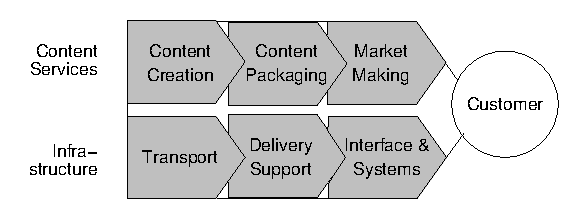
\includegraphics[width=0.4\textwidth]{indica_model}
    \caption{INDICAn kaksitasoinen arvomalli.}
    \label{fig:indica_model}
  \end{center}
\end{figure}

Periaatteessa samaan kelluvaan objektiin voi laittaa useammankin kuvan
(kuva~\ref{fig:tuplat}) tai asetella niitä taulukoilla.
Jos tarvitset useita kuvia rinnakkain, harkitse
myös pakettia \verb!subfigure!.

\begin{figure}[htb]
  \begin{center}
    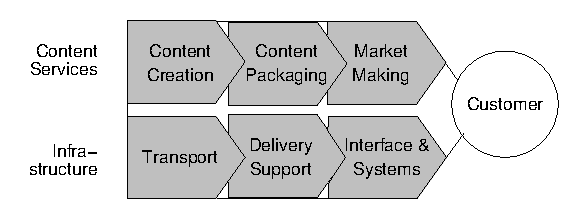
\includegraphics[width=0.32\textwidth]{indica_model}
    %\hfill  % toinen vas. reunaan, toinen oikeaan
    \hspace{10mm}  % sentti väliä kuville
    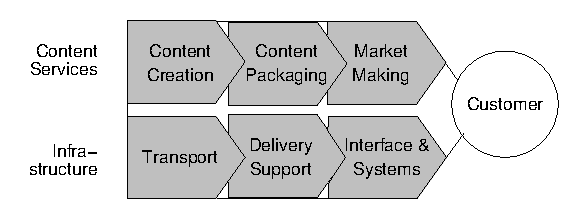
\includegraphics[width=0.25\textwidth]{indica_model}
    \caption{Kaksi kuvaa rinnan esimerkkinä.}
    \label{fig:tuplat}
  \end{center}
\end{figure}

Yksinkertainen taulukko, joka ei ole kelluva ja siten sen pitäisi
latoutua heti tämän tekstin alle. Tässä komento \verb!\topcaption!
kyllä varaa itselleen ``Taulukko 1'', mutta tekstiä ei näy missään.

\topcaption{Yksinkertainen taulukko}
%\begin{center}                         % keskitys?
\begin{tabular}{|l|l|l|} 
\hline
Tässä & sarakkeet & ei ole eroteltu mitenkään \\
ja    & ne        & saattavat valua yli laidankin ikävästi \\
\hline
\end{tabular}
%\end{center}

Toinen kelluva perustaulukko, viitataan nyt taulukkoon~\ref{table:perustaulu}.
Lähdetekstiä lukiessa näet tilde-merkin, joka pakottaa välilyönnin
mutta estää rivinvaihdon.

\begin{table}[ht]
\caption{Tässä perustaulukko.}
\label{table:perustaulu}
\begin{center}
\begin{tabular}{|l|l|l|} 
\hline
Tässä & sarakkeet & ei ole eroteltu mitenkään \\
\hline
ja    & ne        & saattavat valua yli laidankin ikävästi, %
                   siksi käytä taulukkoa~\ref{table:dvbt_param}. %
                   Teksti katoaa jonnekin sivun ulkopuolelle. \\
\hline
Nro   & Nro       & Nro \\
\hline
$-4$  & $8$       & $12$ \\
\hline
\end{tabular}
\end{center}
\end{table}

Vielä kolmas esimerkki taulukosta, jossa sarakkeiden leveys määritelty
ja soluissa voi olla useampi rivi tekstiä. Katso
taulukko~\ref{table:dvbt_param}.

\begin{table}[th]
\caption{The DVB-T transmission parameters.}
\label{table:dvbt_param}
\begin{center}
\begin{tabular}{|p{0.35\textwidth}|p{0.45\textwidth}|} 
    \hline
Parameter & Typical values \\
    \hline
    \hline
Physical channel&8 MHz (also 6 MHz or 7 MHz possible)\\ 
    \hline
COFDM mode (number of subcarriers, 
subcarrier width, 
signal element length)
&8k (6817, 1116 Hz, 896 $\mu$s) or 
2k (1705,4464 Hz, 224 $\mu$s)\\
    \hline
Guard interval (8k/4k duration)
&1/4 (224/56 $\mu$s), 1/8 (112/28 $\mu$s),
   1/16 (56/14 $\mu$s) or 1/32 (28/7 $\mu$s)\\
    \hline
Inner code rate &1/2, 2/3, 3/4, 5/6 or 7/8\\
    \hline
Signal  element constellation 
&QPSK, 16-QAM or 64-QAM \\
    \hline
\end{tabular}
\end{center}
\end{table}


% Tässä esimerkki monisivuisesta taulukosta.
% EI toiminut aivat täydellisesti 27.1.2011: tablecaption hyppäsi edelliselle
% sivulle ennen ylläolevaa taulukkoa. Tämä supertabular taas ei voi olla 
% table-ympäristössä, kun muuten ei sivutu. supertabular on vain tabular,
% joka pitää kirjaa milloin sivun vaihto ja lisää automaatigisesti \end{tabular}
% ja uudestaa \begin{tabular}.
%\begin{center}
%\tablecaption{Esimerkki monisivuisesta taulukosta.}
%%\topcaption{taulukon nimi ylhäällä}
%%\bottomcaption{taulukon nimi alhaalla}
%\tablefirsthead{\hline \# & Sarakkeen aihe \\ \hline \hline }
%\tablehead{\hline \multicolumn{2}{|l|}{jatkoa edelliseltä sivulta} \\ %
%  \hline  \# & Sarakkeen aihe  \\ \hline \hline }
%\tabletail{\hline \multicolumn{2}{|r|}{jatkuu seuraavalle sivulle} \\ \hline}
%\tablelasttail{\hline}
%\label{table:pitkataulukko}
%\begin{supertabular}{|>{\bf}r|p{120mm}|} 
%\hline
%\multicolumn{2}{|l|}{Otsikko A} \\ 
%\hline
%1 & complex numbers, Carthesian and polar coordinate systems, Euler's formula   %\\
%2 & Euler's formula, cosine and sine, odd and even functions   \\
%3 & complex numbers, graphical notation   \\
%\hline 
%\multicolumn{2}{|l|}{Otsikko B} \\ 
%\hline
%14 & analog, discrete-time and digital signal   \\
%17 & analog, discrete-time and digital signal   \\
%16 & digital signals and spectra, spectogram \\
%17 & Fourier series, Fourier transforms: CTFT, DTFT, DFT \\
%18 & time-frequency-domain analysis and filtering \\
%21 & moving average (MA) filter, a simple FIR filter   \\
%22 & a simple IIR filter \\
%23 & flow / block diagram of a discrete-time system   \\
%24 & recognition of LTI systems, causal LTI systems, filter order, FIR, IIR   %\\
%25 & properties of LTI systems: linear, time-invariant, causal, stable   \\
%26 & shifted and scaled sequences in LTI system   \\
%31 & convolution as products of polynomials   \\
%32 & deconvolution   \\
%33 & parallel and cascade (series) LTI systems   \\
%34 & matched filter   \\
%35 & auto- and cross-correlation   \\
%37 & spectrum, CTFT, discrete-time Fourier transform (DTFT), %
% discrete Fourier transform (DFT)   \\
%38 & DTFT, computation from definition   \\
%39 & DTFT, using a transform table   \\
%40 & $2\pi$-periodic spectrum, DTFT   \\
%41 & magnitude/amplitude response, periodicity of DTFT   \\
%43 & sampling, Shannon's theorem   \\
%44 & impulse train and Fourier-series   \\
%45 & impulse train and sampling in frequency-domain   \\
%46 & sampling in frequency-domain   \\
%47 & aliasing   \\
%48 & sampling, aliasing, anti-aliasing   \\
%49 & anti-aliasing filter  \\
%51 & circular shift, DFT \\
%54 & amplitude response grafically from pole-zero-plot   \\
%55 & analysis of LTI IIR system, pole-zero plot   \\
%56 & transfer function, region of convergence (ROC)   \\
%57 & scaling factor   \\
%63 & direct form (DF) structures   \\
%70 & FIR-window method in digital filter design   \\
%71 & computational comparisons between IIR and FIR filters   \\
%73 & FFT computational complexity   \\
%74 & radix-2 DIT FFT algorithm   \\
%75 & binary addition and substraction, two's complement  \\
%78 & roundoff noise in FIR filters   \\
%79 & signal-to-noise ration (SNR) \\
%80 & error-feedback structure   \\
%81 & up- and downsampling in time- and frequency domain   \\
%82 & multirate system analysis   \\
%83 & linearity of up- and downsampling systems   \\
%84 & filter bank   \\
%85 & interpolated FIR filter (IFIR), FIR window method design  \\
%\end{supertabular}
%\end{center}


\subsection{Matematiikka}
\label{sec:esimmatematiikka}

Lyhyet matemaattiset kaavat voi kirjoittaa tekstin
sisään $E_{\textrm{total}} = m_i c^2$, mutta kaavat, joita käytetään, 
kannattaa keskittää
%
\begin{equation}
\label{eq:kaava1}
x^2 + y^2 = 1 
\end{equation}
%
josta lyhyempi versio ilman kaavan numerointia
%
\[ x^2 + y^2 = 1 \]
%
tai jakaa useammalle riville
\begin{equation}
\label{eq:kaava2}
\begin{aligned}
x^2 + y^2 &= 1 \\
        x &= \sqrt{1-y^2}
\end{aligned}
\end{equation}
%

Kreikkalaiset kirjaimet löytyvät taulukosta~\ref{table:kreikka}.

\begin{table}
\caption{Kreikkalaiset kirjaimet}
\label{table:kreikka}
\begin{center}
\begin{tabular}{|llllllll|}
\hline
$\alpha$        &$\theta$       &o              &$\tau$         &%
$\beta$         &$\vartheta$    &$\pi$          &$\upsilon$     \\
$\gamma$        &$\gamma$       &$\varpi$       &$\phi$         &%
$\delta$        &$\kappa$       &$\rho$         &$\varphi$      \\
$\epsilon$      &$\lambda$      &$\varrho$      &$\chi$         &%
$\varepsilon$   &$\mu$          &$\sigma$       &$\psi$         \\
$\zeta$         &$\nu$          &$\varsigma$    &$\omega$       &%
$\eta$          &$\xi$          &               &               \\
\hline
$\Gamma$        &$\Lambda$      &$\Sigma$       &$\Psi$         &%
$\Delta$        &$\Xi$          &$\Upsilon$     &$\Omega$       \\
$\Theta$        &$\Pi$          &$\Phi$         & & & & &       \\
\hline
\end{tabular}
\end{center}
\end{table}

Matematiikkaan liittyviä ohjeistusta löytyy esim. \citet{lyhyt2e}.
Makroja sisältävästä tiedostosta \verb!makroja.tex! löytyy joitakin
esimerkkejä, kuten 
%
\[ \myInt{-\infty}{0}{e^{x}}{x} \]
%

\subsection{Viittaukset ja lähdeluettelo}
\label{sec:esimviitteet}


\subsubsection{Ristiinviittaukset}
\label{sec:esimristiviite}

Ristiinviittauksia taulukkoon, kuvaan, kappaleeseen tai muuhun voi
tehdä \verb!ref!-komennolla, kuten tässä
kuvaan~\ref{fig:indica_model}.  Isossa työssä voi olla näppärä antaa
selailun nopeuttamiseksi myös sivunumero: kuva~\ref{fig:indica_model}
löytyy sivulta~\pageref{fig:indica_model}. Tilde-merkki pakottaa
välin, mutta sitoo sen niin, etteivät ne esiinny eri riveillä.

Johdantoluvun lopussa tyypillisesti esitellään kirjan rakenne, joten
voi viitata, että luvussa~\ref{sec:esimluettelo} tarkastellaan sitä ja
tätä, luvussa~\ref{sec:esimtekstiviite} tuotakin. Englanniksi
kirjoitettaessa isolla etukirjaimella ``Figure~\ref{fig:indica_model} on
page~\pageref{fig:indica_model}'' ja ``Section~\ref{sec:esimtekstiviite}''.


\subsubsection{Lähdetiedosto}
\label{sec:esimlahdetiedosto}

Lähdeluettelo kirjoitetaan joko käsin tai automaattisesti
kerätyistä lähteistä bib-päätteiseen tiedostoon. Katso 
esimerkkejä tiedostosta \verb!lahteet.bib!, jota kutsutaan
\verb!main.tex! tiedoston loppupuolella. 

Kirjaa tiedot mahdollisimman täydellisesti. Kiinnitä erityisesti
huomio nimiin ja kirjoita ne samanmuotoisesti
\verb!Sukunimi, Etunimi and Sukunimi2, Etunimi2 Etukirjain2.!.

Jos esimerkiksi kirjojen nimissä on muotoiluja, pakkaa ne
kaarisulkuihin \verb!{My {T}hesis}!. 
Pelkkä \verb!title={My Thesis}! muuttuu muuten
muotoon ``My thesis''.

Kurssilla opetetaan käyttämään RefWorksia lähteiden kokoamiseen.
Sieltä on mahdollista saada BibTeX-muotoinen luettelo lähteistä.
Valitse ylävalikosta ``Bibliography'' ja ensimmäisellä kerralla
valitse alasvetovalikosta ``Access output style manager'' ja
sieltä lisää BibTeX suosikkeihin. Määrää lähdetiedosto tekstityyppiseksi
(``Text'') ja luo tiedosto. RefWorksin tulostukseen tulee loppuun
ylimääräinen sulkumerkki \verb!}!, viimeisen tietorivin perässä
ylimääräinen pilkku ja alusta puuttuu itse viittausnimi, jonka
voit itse keksiä.

Google Scholar palauttaa myös BibTeX-muotoisia lähdeviitteitä,
kunhan olet sen asetuksissa valinnut BibTeXin mahdolliseksi.

\subsubsection{Tekstiviite}
\label{sec:esimtekstiviite}

Tässä pohjassa käytetään (ilmeisesti) Helsingin yliopiston 
\verb!tktl!-tyyliä, joka pohjautuu \verb!natbib!-tyyliin.
Tekstiviitteet saadaan mukaan joko tekijä-vuosi-tavalla (oletusarvo)
tai yksinkertaisella numeromerkinnällä, kuten \verb![1]!. 
Jälkimmäistä varten sinun pitää vaihtaa tekstiviitteen esitystapa
tiedon \verb!main.tex! lopussa rivillä \verb!bibpunct!. 

% kokeillaan vähän vapaampaa, kun natbibiin kohdalla rivivaihto
\begin{sloppypar}
Katso eri tapoja tekstiviitteiden muotoiluun sivulta
\url{http://merkel.zoneo.net/Latex/natbib.php}.
Viittauskomennot  \verb!\citet! ja \verb!\citep! ovat
hyviä tekijä-vuosi-tavassa \verb!natbib!iin liittyen
ja \verb!\cite! on perusviittauskomento.
\end{sloppypar}

Pari esimerkkiä:
Usein selitetetään, että~\citet[s. 21]{Teekkari2010} on 
havainnut asian jos toisenkin. 
Tämä ja tuo uusi havainto on vahvistanut teoriaa~\citep[s. 22]{Teekkari2010}.
Joku asia on selitetty tarkasti monissa lähteissä 
\citep[katso][s. 27]{Teekkari2010}.


\subsubsection{Lähdeluettelo}
\label{sec:esimlahdeluettelo}

Lähdeluettelon tulisi nyt ilmaantua dokumentin loppuun
automaattisesti. Jos sitä ei näy ja etenkin jos tekstiviitteiden
paikalla on kysymysmerkkejä, niin muista ajaa \verb!bibtex main!.

% --------------------------------------------------------------------

\section{Tekstin osat}
\label{sec:tekstin_osat}

Suomen kielen lehtori Sanni Heintzmann kirjoitti tammikuussa 2011
ohjeistusta seuraavista kandidaatintyön luvuista tai osista:
alkusanat, käytetyt lyhenteet, johdanto, loppuluku ja tiivistelmä.

\subsection{Alkusanat}

Alkusanoissa voi kiittää tahoja, jotka ovat merkittävästi edistäneet
työn valmistumista. Tällaisia voivat olla esimerkiksi yritys, jonka
tietokantoja, kontakteja tai välineistöä olet saanut käyttöösi,
haastatellut henkilöt, ohjaajasi tai muut opettajat ja myös
henkilökohtaiset kontaktisi, joiden tuki on ollut korvaamatonta työn
kirjoitusvaiheessa. Alkusanat jätetään tyypillisesti pois
kandidaatintyöstä, joka on laajuudeltaan vielä niin suppea, ettei
kiiteltäviä tahoja luontevasti ole.

\textbf{TIK.kand suositus: Älä käytä tällaista lukua.}

\subsection{Käytetyt lyhenteet}

Tähän voidaan listata kaikki työssä käytetyt lyhenteet. Lyhenteistä
annetaan selityksenä sekä alkukielinen termi kokonaisuudessaan
(esim. englanninkielinen lyhenne avattuna sanoiksi) että sama
suomeksi. Jos suoraa käännöstä ei ole tai sellaisesta on vaikea saada
sujuvaa, voi käännöksen sijaan antaa selityksen siitä, mitä kyseinen
käsite tarkoittaa. Jos lyhenteitä ei esiinny työssä paljon, ei tätä
osiota tarvita ollenkaan. Yleensä luettelo tehdään, kun lyhenteitä on
10-20 tai enemmän. Vaikka lyhenteet annettaisiinkin tässä
keskitetysti, ne pitää silti avata sekä suomeksi että alkukielellä
myös itse tekstissä, kun ne esiintyvät siellä ensi kertaa.  Käytetyt
lyhenteet -osion voi nimetä myös ''Käytetyt lyhenteet ja termit'', jos
luettelossa on sekä lyhenteitä että muuta käsitteenmäärittelyä.

\textbf{TIK.kand suositus: Käytä vasta kun lyhenteitä yli 10.}

\textbf{TIK.kand suositus: Lisää lyhenne- tai symbolisivu, kun se
  näyttää luontevalta ja järkevältä.}

\subsection{Johdanto}

Työn ensimmäinen luku on aina johdanto. Kandidaatintyön laajuudessa
sitä ei ole tarvetta jakaa alalukuihin, diplomityössä ja muissa
isommissa töissä sekä tutkimusraporteissa alaluvut ovat mahdollisia
(esim. 1.1 Tutkimusongelma, 1.2 Aineisto ja tutkimusmenetelmä, jne.).

Johdannon tarkoitus on antaa lukijalle heti alussa selvä kuva siitä,
mihin kysymykseen työ pyrkii vastaamaan
(tutkimusongelma). Tyypillisesti aiheen esittely alkaa sanoilla ''Tämä
(kandidaatin/diplomi)työ käsittelee...'' Johdanto esittelee lyhyesti
työn pääpiirteet ja johdattaa lukijan itse työn pariin. Johdannon
ohjepituus on 1--3 sivua, kandidaatintyössä 2 sivua on hyvä maksimi.

Käsittele nämä aiheet johdannossa (jotakuinkin tässä järjestyksessä):
\begin{itemize}
 \item Johdatus aihepiiriin (ei liian laajasti, vaan relevantisti ja napakasti)
%
 \item Tutkimuskohteen esittely (MITÄ tämä työ tutkii? 
Kerro työstä/tutkimusaiheesta, ei omasta kirjoitusprosessistasi 
tai omasta kiinnostuksestasi.)
%
 \item Tutkimuksen perustelu: ongelma tai aukko 
(aiemmassa tutkimuksessa on aukko, tai siitä nousee esiin 
kysymys, johon tässä etsitään vastausta)
%
 \item Tutkimusongelma / -kysymykset (koko työsi sydän, 
jonka pitäisi näkyä ''punaisena lankana'' koko työn läpi)
 \item Tavoitteet (Käytä konkreettisesti sanaa ''tavoite'')
 \item Rajaus (Mitä tämä työ EI tutki)
 \item Menetelmä, aineisto, teoreettinen kehys (Esittele, 
MITEN em. aihetta tutkitaan)
 \item Tulokset? (Johdannossa on ihan hyvä antaa lyhyesti 
tietoa päätuloksista, mutta ei pakko)
 \item Työn sisältö ja rakenne (Esittele, miten työn punainen 
lanka etenee, viittaukset työhön: 
``ensin, sitten, seuraavaksi, luvussa 3'' jne.)
\end{itemize}

\subsection{Loppuluku}

Loppuluku päättää työn. Luvun nimi on tyypillisesti ``yhteenveto'' tai
``johtopäätöksiä''. Valitse se otsikko, joka tuntuu sopivammalta työsi
luonteeseen. Joka tapauksessa loppuluku sisältää niin työn yhteenvedon
kuin johtopäätöksiä työn tulosten perusteella. Pääajatus on antaa
lukijalle selvä kuva siitä, miten johdannossa asetettuihin
tavoitteisiin työssä vastattiin.

Käsittele loppupuvussa seuraavia asioita (jotakuinkin tässä järjestyksessä):
%
\begin{itemize}
  \item Muistutus työn tavoitteista (sidoksisuus johdantoon)
  \item Päätulokset kootaan yhteen, pohditaan niiden merkitystä
  \item Suositukset konkreettisiksi toimenpiteiksi (``Mitä sitten?'' 
Nyt kun käytössä on tämän työn myötä tullut tieto, 
mitä se nyt tarkoittaa tälle asialle/alalle.)
  \item Tulosten soveltuvuus, käyttöön liittyvät rajoitukset
  \item Jatkotutkimustarve 
(``Tulevaisuudessa olisi mielenkiintoista selvittää...'' tms.)
  \item Työn onnistumisen arviointi 
(Huom! Älä arvioi omaa kirjoitusprosessiasi vaan tekemääsi tutkimusta)
\end{itemize}

\subsection{Tiivistelmän kirjoitusohjeita}

Tiivistelmä on muusta työstä täysin irrallinen teksti, joka
kirjoitetaan tiivistelmälomakkeelle vasta, kun koko työ on valmis. Se
on suppea ja itsenäinen teksti, joka kuvaa olennaisen opinnäytteen
sisällöstä. Tavoitteena selvittää työn merkitys lukijalle ja antaa
yleiskuva työstä. Tiivistelmä markkinoi työtäsi potentiaalisille
lukijoille, siksi tutkimusongelman ja tärkeimmät tulokset kannattaa
kertoa selkeästi ja napakasti. Tiivistelmä kirjoitetaan hieman
yleistajuisemmin kuin itse työ, koska teksti palvelee
tiedonvälitystarkoituksessa laajaa yleisöä.

Tiivistelmän rakenne:
\begin{itemize}
%
\item Teksti jäsennetään kappaleisiin (3--5 kappaletta)
\item Ei väliotsikkoja
\item Ei mitään työn ulkopuolelta
\item Ei tekstiviitteitä tai lainauksia
\item Vähän tai ei ollenkaan viittauksia työhön 
(ei ollenkaan: ``luvussa 3'' tms., mutta koko työhön voi 
viitata esim. sanalla ``kandidaatintyössä'')
\item Ei kuvia ja taulukoita
\item Löysät pois: 	 
  \begin{itemize}
    \item Ei työn rakenteen esittelyä
    \item Ei itsestäänselvyyksiä
	 \item Ei turhaa toistoa
    \item Älä jätä lukijaa nälkäiseksi, eli kerro asiasisältö, 
älä vihjaa, että työssä kerrotaan se.
  \end{itemize}
\item Tyypillinen rakenne: 
  \begin{itemize}
    \item[1.] Aihe, tavoite ja rajaus 
(heti alkuun, selkeästi ja napakasti, ei johdattelua)
    \item[2.] Aineisto ja menetelmät (erittäin lyhyesti)
    \item[3.] Tulokset (tälle enemmän painoarvoa)
    \item[4.] Johtopäätökset (tälle enemmän painoarvoa)
  \end{itemize}
\end{itemize}

\textbf{TIK.kand suositus: Tiivistelmä kirjoitetaan vasta kun työ on tehty.}

% --------------------------------------------------------------------

% Tätä käytetään vain testaustarkoituksiin, kun halutaan katsoa 
% miten sivu täyttyy pelkästä tekstistä. Teksti haettu eduskunta.fi-sivustolta
% tammikuussa 2011.

\section{Testi: pelkkää tekstiä}

Eduskunnan ympäristövaliokunta ehdottaa, että nykyinen
hajajätevesiasetus kumotaan ja ympäristöministeriö laatii uuden
asetuksen mahdollisimman pian. Lisäksi valiokunta ehdottaa, että
ympäristönsuojelulakiin sisällytetään uusi 3 a luku, johon tulee
yhteensä 5 pykälää. Ympäristövaliokunta antoi asiaa koskevan mietinnön
25. tammikuuta (YmVM 18/2010).

Valiokunta esittää lisäksi eduskunnan hyväksyttäväksi viisi
lausumaehdotusta, joilla vauhditetaan lain ja uuden asetuksen selkeää
ja tehokasta toimeenpanoa. Nyt esitettävät muutokset on valmisteltu
tiiviissä yhteistyössä ympäristöministeriön
kanssa. Ympäristövaliokunta on käsitellyt asiaa laajasti ja
perusteellisesti sekä ottanut ehdotuksissaan huomioon sen, mitä
perustuslakivaliokunta aiemmin asiassa edellytti.

Ehdotetuilla muutoksilla kohtuullistetaan hajajätevesien käsittelyn
vaatimustasoa siten, että vaatimukset asettuvat yleisesti sellaiselle
tasolle, että ne ovat kohtuullisella investoinnilla ja toimivalla
tekniikalla moitteettomasti täytettävissä. Esitetty kohtuullistaminen
ei kuitenkaan vaaranna ympäristönsuojelun tasoa ja on esimerkiksi
Itämeren suojelukomissio HELCOMin suositusten mukainen.

Nykyisen asetuksen lievempi vaatimustaso (orgaaninen aine 80\%,
kokonaisfosfori 70\%, kokonaistyppi 30\%) säädetään pääsääntöisesti
noudatettavaksi lähtökohdaksi, koska suuri osa kiinteistöistä
sijaitsee muualla kuin herkillä alueilla kuten ranta-alueella. Kunnat
voivat kuitenkin ympäristönsuojelumääräyksillä antaa tiukempia
määräyksiä ympäristön pilaantumisvaaran perusteella herkillä alueilla
kuten ranta-alueilla tai tärkeillä pohjavesialueilla.

Puhdistustasovaatimuksen perusteista säädetään laissa ja prosentit
edelleen asetuksella. Uudet säännökset ovat ensisijaisesti
jätevesijärjestelmän suunnittelun ja rakentamisen lähtökohta, eivät
valvontaperuste. Tosiasiallinen puhdistustulos voi siten vaihdella
esimerkiksi sääoloista tai kiinteistön käytön väliaikaisista
muutoksista johtuen, ja silti järjestelmä täyttää lain vaatimukset.

Valiokunta korostaa, että lain ja asetuksen mukaisten vaatimusten
toteuttaminen käytännössä edellyttää aina kiinteistökohtaista
arviointia. Kiinteistökohtainen neuvonta on siksi järjestettävä
valtakunnallisessa ohjauksessa. Valiokunta edellyttää riittävää
määrärahaa neuvonnan järjestämiseksi kunnissa.  Vaatimustason
muutoksella kohtuullistetaan tarvittavia investointeja, mutta
säilytetään samalla riittävä ympäristönsuojelun taso. Erityisen
tärkeää on ehkäistä lähiympäristön kuten kaivoveden pilaantumista ja
muita vastaavia hygieenisiä haittoja.

Muutoksella vapautetaan suoraan lain nojalla lain voimaan tullessa 68
vuotta täyttäneet vakituisesti asuttujen kiinteistön haltijat
asetuksen käsittelyvaatimuksista. Vapautus ei koske uudisrakentamista
eikä vapaa-ajan asuntoja. Käytännössä toimenpiteitä tarvitaan
vesivessalla varustetuilla vapaa-ajan asunnoilla.  Valtaosalla
vapaa-ajan asuntoja lainsäädäntö ei aiheuta mitään toimenpiteitä.

Muutoksella tarkennetaan, ketkä voivat hakea kunnalta viiden vuoden
mittaista vapautusta asetuksen vaatimusten noudattamisesta niin
sanotun sosiaalisen suoritusesteen (erityisen vaikeassa
elämäntilanteessa olevat kiinteistönomistajat kuten työttömät ja
pitkäaikaissairaat) perusteella.  Lainmuutos ja uusi asetus voivat
tulla voimaan 15.3.2011. Jo rakennetun kiinteistön olemassa olevan
jätevesijärjestelmän on täytettävä puhdistustehosta asetetut
vaatimukset vuoteen 2016 mennessä.

Suomen Euroopan neuvoston valtuuskunnan jäsenet Kimmo Sasi (kok.) ja
Krista Kiuru (sd.) vaativat parlamentaarisen yleiskokouksen
istunnossa, että Kosovossa rikosten uhreina kadonneiden ihmisten
kohtalot selvitetään.

Yleiskokous käsitteli tiistaiaamuna etukäteen paljon huomiota
herättänyttä sveitsiläisen kansanedustajan Dick Martyn raporttia
Kosovon vuoden 1999 sodan jälkimainingeissa tapahtuneista
ihmisoikeusloukkauksista. Martyn mukaan Kosovon vapautusarmeija
surmasi vangeiksi ottamiaan ihmisiä, poisti heiltä elimiä ja kauppasi
niitä pimeillä markkinoilla.

Keskustelussa Martyn väitteet myös kiistettiin. Kansanedustaja Krista
Kiuru korostikin täysistuntopuheessaan, että väitteet pitää tutkia
huolellisesti.  Totuuden selvittämiseksi tarvitaan puolueeton ja
läpinäkyvä tutkinta kansallisten ja kansainvälisten viranomaisten
yhteistyönä, hän totesi.  Kansanedustaja Kimmo Sasi (kok.) piti
huolestuttavana, että satojen ihmisten epäillään kadonneen sodan
jälkimainingeissa rikoksen uhreina.

Tarpeellisia selvityksiä ei voida tehdä ilman Albanian ja Kosovon
täydellistä yhteistyötä. Euroopan neuvoston pitääkin varmistaa, että
selvityksiä ei estetä tai vaikeuteta poliittisista syistä. Kosovon
hallitukselle onkin tärkeää, että asia tutkitaan. Vaikeidenkin
historian tapahtumien täydellinen läpikäynti auttaa rakentamaan
parempaa tulevaisuutta. Osoittamalla olevansa vahva oikeusvaltio,
vahvistaa Kosovo omaa asemaansa itsenäisenä valtiona, Sasi totesi.

Eduskunta korjaa pikavauhtia neljän kansanedustajan lakialoitteella
metsälakiin jääneen virheen, jonka takia pienet taimikot jäivät
tilapäisesti hirvivahinkokorvausten ulkopuolelle.  Metsälain muutos
tuli voimaan vuoden vaihteessa. Maa- ja metsätalousministeriössä lain
valmistelussa tapahtuneen teknisen virheen takia pienet, alle 1,3
metrin pituiset taimikot jäivät lakimuutoksen myötä hirvivahinkojen
korvauksen ulkopuolelle.  Lakitekstiin kiireessä jäänyt virhe
havaittiin vasta, kun laki oli jo hyväksytty ja vahvistettu, mitä
ministeriö pahoitteli. Virhe korjataan eduskunnan maa- ja
metsätalousvaliokunnan puheenjohtajan Jari Lepän (kesk.)
lakialoitteella, jonka on allekirjoittanut myös kolme muuta
valiokunnan kansanedustajaa.

Aloitteen tekijät ehdottavat, että kyseistä riistavahinkolain pykälää
korjattaisiin siten, että lakia sovellettaisiin taannehtivasti vuoden
alusta alkaen. Siten kukaan ei lopullisesti menetä oikeuttaan
korvaukseen.  Lakialoite (LA 121/2010) oli lähetekeskustelussa
tiistaina. Keskustelun päätteeksi asia lähetettiin maa- ja
metsätalousvaliokuntaan.

Euroopan unionin ympäristömerkki siirtyy samaan kotipesään
pohjoismaisen Joutsenmerkin kanssa. Eduskunta hyväksyi tiistaina
lakimuutoksen, jolla ympäristömerkinnän kansallisten tehtävien hoito
siirtyy Suomen Standardisoimisliitolta Motiva Services Oy:lle.
Suomessa on käytössä kaksi virallista
ympäristömerkintäjärjestelmää. Pohjoismainen ympäristömerkki eli
Joutsenmerkki on Pohjoismaiden ministerineuvoston vuonna 1989
perustama merkki. EU:n ympäristömerkki on Euroopan parlamentin ja
neuvoston antamaan asetukseen pohjautuva ympäristömerkki.

Merkit ovat vapaaehtoisia ja niillä kannustetaan valmistajia ja
palvelutarjoajia kehittämään ympäristön kannalta parempia
vaihtoehtoja. Joutsenmerkkejä on myönnetty yli 300. EU:n
ympäristömerkin luvanhaltijoita on noin 10 ja merkittyjä tuotteita
noin 50.  Joutsenmerkin hallinnointi siirtyi Motivalle vuoden
vaihteessa. Motiva Services Oy on valtion omistama asiantuntijayritys,
joka edistää energian ja materiaalien tehokasta ja kestävää käyttöä.

% --------------------------------------------------------------------


%\clearpage                     % luku loppuu, loput kelluvat tänne, sivunv.

\label{pages:text}
%\clearpage                     % luku loppuu, loput kelluvat tänne, sivunv.

%\newpage                       % pakota lähdeluettelo alkamaan uudelta s.

% -------------- Lähdeluettelo / reference list -----------------------
%
% Muista, että saat kirjallisuusluettelon vasta
%  kun olet kääntänyt ja kaulinnut "latex, bibtex, latex, latex"
%  (ellet käytä Makefilea ja "make")

% Viitetyylitiedosto aaltosci_t.bst; muokattu HY:n tktl-tyylistä.
% Pakettiin natbib liittyen katso esim. 
% http://merkel.zoneo.net/Latex/natbib.php
% jossa selitykset citep, citet, bibpunct, jne.
\bibliographystyle{aaltosci_t}
\bibpunct{(}{)}{;}{a}{,}{,}    % a = author-year
%\bibpunct{[}{]}{;}{n}{,}{,}    % n = numerical style

% Muutetaan otsikko "Kirjallisuutta" -> "Lähteet"
\renewcommand{\refname}{Lähteet}  % article-tyyppisen
%\renewcommand{\bibname}{Lähteet}  % jos olisi book, report-tyyppinen

% Lisätään sisällysluetteloon
\addcontentsline{toc}{section}{\refname}  % article
%\addcontentsline{toc}{chapter}{\bibname}  % book, report

% Määritä kaikki bib-tiedostot
\bibliography{lahteet}
%\bibliography{thesis_sources,ietf_sources}

\label{pages:refs}
\clearpage         % erotetaan mahd. liitteet alkamaan uudelta sivulta

% -------------- Liitteet / Appendices --------------------------------
%
% Liitteitä ei yleensä tarvita. Joskus matemaattisen kaavan
%  tarkempi johtaminen, haastattelurunko, kyselypohja, 
%  ylimääräisiä kuvia, lyhyitä ohjelmakoodeja tai datatiedostoja.
%
%\appendix
%\section{Esimerkkiliite}
\label{sec:app1}

Ei normaalisti liitteitä. Joskus liitteeksi lisätään matemaattisen kaavan
tarkempi johtaminen, haastattelurunko, kyselypohja, 
ylimääräisiä kuvia, lyhyitä ohjelmakoodeja tai datatiedostoja.

Työtä varten mahdollisesti tehtyjä ohjelmakoodeja ei tyypillisesti
lisätä tänne, ellei siihen ole joku erityinen syy. (Kukaan ei ala kirjoittaa koodia paperilta vaan pyytää sitä sinulta, jos on kiinnostunut.)

Toiset ohjeet kertovat, että liitteet tulisi numeroida omilla sivunumeroillaan. Voit käyttää myös tekstiosasta jatkuvaa numerointia.

\subsection{Esimerkkiliitteen otsikko 1}
\label{sec:app1_1}

Kerätty data-aineisto.

\section{Toinen esimerkkiliite}
\label{sec:app2}

Haastattelukysymykset: mitä, missä, milloin, kuka, miten.


\label{pages:appendices}

\end{document}
